\section{Auswertung}
\label{sec:Auswertung}

\subsection{Bestimmung der maximalen magnetischen Kraftflussdichte}
Die mit Hilfe einer Hallsonde bestimmten Messwerte sind in \autoref{tab:bfeld} eingetragen und wurden in
\autoref{fig:plot} graphisch dargestellt. Die maximale Feldstärke lässt sich zu $\SI{422}{\milli\tesla}$
bei $x=\SI{89}{\milli\meter}$ oder $x=\SI{90}{\milli\meter}$ ablesen. Um das Maximum verlässlich ablesen
zu können, wurden um das Maximum mehr Messwerte aufgenommen.

\begin{table}[hbt!]
  \centering
  \caption{Mit einer Hallsonde im Luftspalt gemessene Feldstärke zur Bestimmung des maximalen Feldstärkewerts.}
  \label{tab:bfeld}
  \begin{tabular}{c c}
    \toprule
    $x/\si{\milli\meter}$ & $B/\si{\milli\tesla}$\\
    \midrule
    $ 70$ & $ 14$ \\
    $ 75$ & $ 72$ \\
    $ 80$ & $309$ \\
    $ 85$ & $415$ \\
    $ 86$ & $416$ \\
    $ 87$ & $419$ \\
    $ 88$ & $421$ \\
    $ 89$ & $422$ \\
    $ 90$ & $422$ \\
    $ 91$ & $420$ \\
    $ 92$ & $416$ \\
    $ 93$ & $411$ \\
    $ 94$ & $403$ \\
    $ 95$ & $396$ \\
    $100$ & $212$ \\
    $105$ & $ 41$ \\
    $110$ & $  9$ \\
    \bottomrule
  \end{tabular}
\end{table}

\begin{figure}[hbt!]
  \centering
  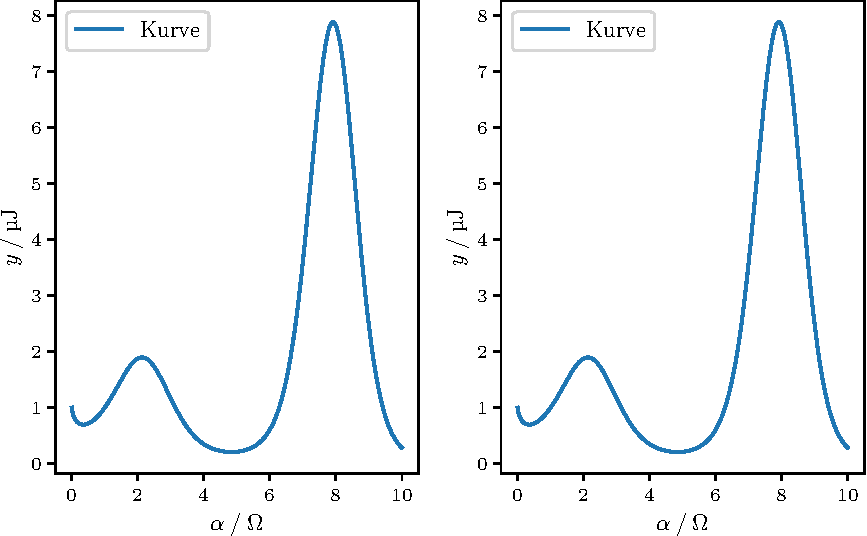
\includegraphics{plot.pdf}
  \caption{Die magnetische Feldstärke $B$ in $mT$ gegen die Koordinate $x$ in $mm$ aufgetragen.}
  \label{fig:plot}
\end{figure}

\subsection{Bestimmung der effektiven Masse}
Es wird Licht mit neun unterschiedlichen Wellenlängen im Bereich von $\SI{1,06}{\micro\meter}$ bis
$\SI{2,65}{\micro\meter}$ verwendet, um die Faraday-Rotation zu bestimmen. Die drei Gallium-Arsenid-Proben haben
die Parameter
\begin{align*}
  d_{\symup{hochrein}} &= \SI{5,11}{\milli\meter}\symup{,} \\
  d_{N=1,2 \cdot 10^{18} \si{cm}^{-3}} &= \SI{1,36}{\milli\meter}\,\symup{ und} \\
  d_{N=2,8 \cdot 10^{18} \si{cm}^{-3}} &= \SI{1,296}{\milli\meter}\,\symup{.}
\end{align*}
Dabei ist die erste Probe undotiert und anderen beiden sind mit einer Dotierkonzentration $N$ n-dotiert.
Die am Goniometer abgelesenen Winkel wurden zur besseren Lesbarkeit in Grad umgerechnet. Weiterhin wurde die
Winkeldifferenzen $\theta = \frac{1}{2}|\theta_{1} - \theta_{2}|$ in Radianten umgerechnet und mit Hilfe
der oben angegebenen Parameter zu $\frac{\theta}{d}$ normiert.
Die entsprechenden Messwerte und bestimmten Größen sind in \autoref{tab:m1}, 3 und 4 zu finden.
\begin{table}[hbt!]
  \centering
  \caption{Messwerte und die daraus bestimmten Größen $\theta$ und $\theta/d$ für die undotiert GaAs-Probe.}
  \label{tab:m1}
  \begin{tabular}{c c c c c}
    \toprule
    $\lambda/\si{\micro\meter}$ & $\theta_{1}/\si{\degree}$ & $\theta_{2}/\si{\degree}$ & $\theta/\symup{rad}$ & $\theta/d/\symup{rad}\, \si{m}^{-1}$\\
    \midrule
    $1,06 $ & $41,13$ & $60,50$ & $0,1690$ & $33,13$ \\
    $1,29 $ & $57,00$ & $41,16$ & $0,1381$ & $27,09$ \\
    $1,45 $ & $45,16$ & $58,08$ & $0,1127$ & $22,10$ \\
    $1,72 $ & $43,50$ & $52,66$ & $0,7999$ & $15,68$ \\
    $1,96 $ & $40,00$ & $46,60$ & $0,5759$ & $11,29$ \\
    $2,156$ & $45,58$ & $40,50$ & $0,4436$ & $ 8,69$ \\
    $2,34 $ & $28,78$ & $33,25$ & $0,3897$ & $ 7,64$ \\
    $2,51 $ & $24,38$ & $28,00$ & $0,3156$ & $ 6,18$ \\
    $2,65 $ & $32,89$ & $37,56$ & $0,4072$ & $ 7,98$ \\
    \bottomrule
  \end{tabular}
\end{table}

\begin{table}[hbt!]
  \centering
  \caption{Messwerte und die daraus bestimmten Größen $\theta$ und $\theta/d$ für die n-dotierte GaAs-Probe
  mit $N=1,2 \cdot 10^{18} \si{cm}^{-3}$.}
  \label{tab:m2}
  \begin{tabular}{c c c c c}
    \toprule
    $\lambda/\si{\micro\meter}$ & $\theta_{1}/\si{\degree}$ & $\theta_{2}/\si{\degree}$ & $\theta/\symup{rad}$ & $\theta/d/\symup{rad}\, \si{m}^{-1}$\\
    \midrule
    $1,06 $ & $23,16$ & $18,00$ & $0,0045$ & $ 8,84$ \\
    $1,29 $ & $24,56$ & $15,83$ & $0,0076$ & $14,94$ \\
    $1,45 $ & $25,83$ & $27,00$ & $0,0010$ & $19,96$ \\
    $1,72 $ & $27,00$ & $18,83$ & $0,0071$ & $13,97$ \\
    $1,96 $ & $27,00$ & $27,33$ & $0,0029$ & $57,03$ \\
    $2,156$ & $23,00$ & $30,08$ & $0,0061$ & $12,12$ \\
    $2,34 $ & $21,99$ & $29,16$ & $0,0062$ & $12,26$ \\
    $2,51 $ & $29,41$ & $21,66$ & $0,0067$ & $13,26$ \\
    $2,65 $ & $29,99$ & $20,41$ & $0,0083$ & $16,39$ \\
    \bottomrule
  \end{tabular}
\end{table}

\begin{table}[hbt!]
  \centering
  \caption{Messwerte und die daraus bestimmten Größen $\theta$ und $\theta/d$ für die n-dotierte GaAs-Probe
  mit $N=2,8 \cdot 10^{18} \si{cm}^{-3}$.}
  \label{tab:m3}
  \begin{tabular}{c c c c c}
    \toprule
    $\lambda/\si{\micro\meter}$ & $\theta_{1}/\si{\degree}$ & $\theta_{2}/\si{\degree}$ & $\theta/\symup{rad}$ & $\theta/d/\symup{rad}\, \si{m}^{-1}$\\
    \midrule
    $1,06 $ & $16,69$ & $4,11$  & $0,0109$ & $21,53$ \\
    $1,29 $ & $14,90$ & $6,00$  & $0,0077$ & $15,22$ \\
    $1,45 $ & $13,30$ & $6,81$  & $0,0056$ & $11,09$ \\
    $1,72 $ & $15,41$ & $8,16$  & $0,0063$ & $12,40$ \\
    $1,96 $ & $20,66$ & $1,106$ & $0,0083$ & $16,42$ \\
    $2,156$ & $23,38$ & $2,705$ & $0,0031$ & $ 6,27$ \\
    $2,34 $ & $22,75$ & $2,838$ & $0,0049$ & $ 9,63$ \\
    $2,51 $ & $24,00$ & $2,900$ & $0,0043$ & $ 8,55$ \\
    $2,65 $ & $26,05$ & $3,058$ & $0,0039$ & $ 7,75$ \\
    \bottomrule
  \end{tabular}
\end{table}
Außerdem wird in \autoref{fig:norm} die normierte Faraday-Rotation $\theta/d$ gegen $\lambda^2$ aufgetragen.
In wird die Differenz der normierten Faraday-Rotation der hochreinen GaAs-Probe und den n-dotierten GaAs-Proben
gegen das Quadrat der Wellenlänge aufgetragen. Um die effektive Masse zu bestimmen, werden zwei Ausgleichsgeraden
für die die Differenzen der normierten Faraday-Rotationen der n-dotierten GaAs-Proben mit der hocheinen bestimmt.
Die Ausgleichsrechnung wird durch
\begin{align*}
  \theta_{frei} = a\cdot \lambda^2 + b
\end{align*}
beschrieben.
Der entsprechende Plot ist in \autoref{fig:diff} finden.
\begin{figure}[hbt!]
  \label{fig:norm}
  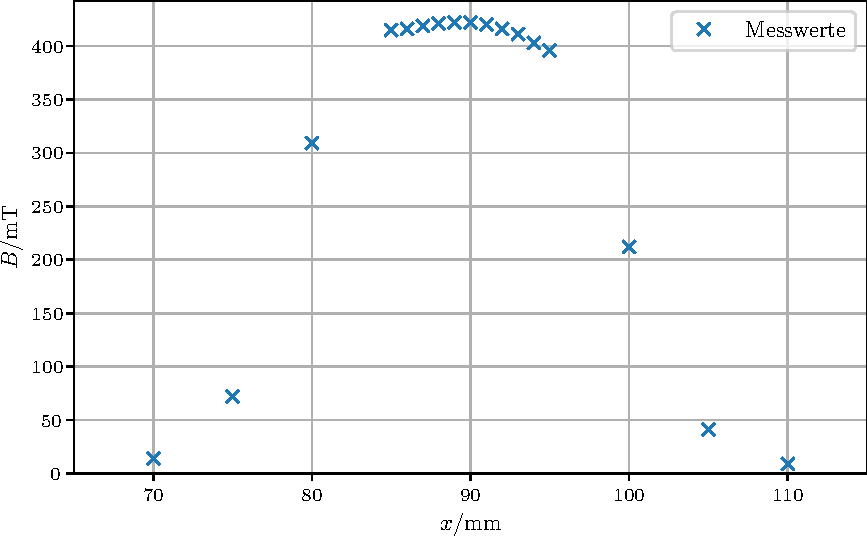
\includegraphics{plot1.pdf}
  \caption{Die normierte Faraday-Rotation $\theta/d$ gegen die quadrierte Wellenlänge $\lambda^2$ für die
  hochreine und den beiden n-dotierten GaAs-Proben.}
\end{figure}

\begin{figure}[hbt!]
  \label{fig:diff}
  \includegraphics{plot2.pdf}
  \caption{Die normierte Faraday-Rotation $\theta/d$ gegen die quadrierte Wellenlänge $\lambda^2$ für die
  hochreine und den beiden n-dotierten GaAs-Proben.}
\end{figure}
\autoref{eq:theta} lässt sich umstellen zu
 \begin{align*}
  m^{*} = \sqrt{\frac{e_0^3}{8\pi^2 \varepsilon_0 c^3} \frac{N B_\text{max}}{n} \frac{1}{a}}
  \end{align*}
Die Parameter der linearen Regression bestimmen sich für die $N=1,2\cdot 10^{18}\,cm^{-3}$ zu
\begin{align*}
  a &= (5264638028593,00 \pm 906926335419,09) \si{\meter}^{-3} \\
  b &= (-25,61 \pm 3,97) \si{\meter}^{-1}
\end{align*}
und für die $N=2,8\cdot 10^{18}\,cm^{-3}$ zu
\begin{align*}
  a &= (2480202027226,74 \pm 711670873463,99) \si{meter}^{-3} \\
  b &= (-13,12 \pm 3,12) \si{meter}^{-1}
\end{align*}